\chapter{Introduction}\label{chap:introduction}

\epigraph{The best that most of us can hope to achieve in physics is simply to misunderstand at a deeper level.}{-- Wolfgang Pauli\footnotemark}

\footnotetext{To Jagdish Mehra, in Berkeley, California (May 1958), as quoted in \emph{The Historical Development of Quantum Theory} (2000) by Jagdish Mehra.}

\section{The Origins of the Chemical Elements}
Atoms are the basic building blocks of matter. Within each atom is a nucleus of protons and neutrons that traces back to its formation at a particular time during the 13.8 billion year history of our universe. Most of the hydrogen and helium nuclei were formed in the high temperature early universe just minutes after the Big Bang. Thereafter, successive generations of stars hosted the nuclear furnaces needed to produce the heavier elements that make up planets, complex molecules, and life. Today, we are continuing to find new applications for the rich set of chemical elements left behind by ancient stars. Our modern computer revolution is taking place only because stars have synthesised elements such as copper, silicon, and literally dozens of metals including gallium and arsenic \citep{Eggert:2008ux}.

The complex processes of stellar nucleosynthesis were first described in detail by \citet{Burbidge:1957hf} and \citet{Cameron:1957jd}. Despite decades of improvements to our theoretical models, there remain large uncertainties in our understanding of processes such as mass loss, convection, and rotation in stars. These uncertainties in stellar physics propagate to uncertainties in our understanding of the universe's chemical enrichment history \citep[see e.g.,][]{Romano:2010hf}. Nevertheless, we currently have a general qualitative understanding of how chemical enrichment takes place.

\begin{figure}
 \begin{center}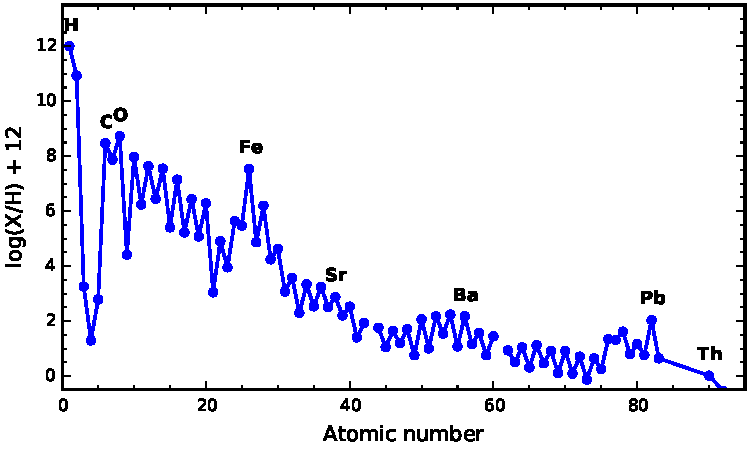
\includegraphics[width=\textwidth]{fig-solarabundances.pdf}\end{center}
 \caption{The solar system abundances by number relative to hydrogen. Data from \citet{Asplund:2009eu}.}\label{fig:solarabund}
\end{figure}

Figure \ref{fig:solarabund} shows the abundances of the chemical elements in the solar system. Broadly, these elements can be classified into: hydrogen and helium created soon after the Big Bang, lithium, beryllium, and boron mostly from cosmic ray spallation, carbon up to iron (Fe) produced by thermonuclear fusion, and elements heavier than the Fe-peak ($Z>30$; hereafter, heavy elements), which are almost entirely produced by neutron captures onto Fe-peak elements. Beyond lead, instability to $\alpha$- and $\beta$-decays prevents further nucleosynthesis via slow neutron captures \citep{Clayton:1967co} and only a very small amount is synthesised via rapid neutron captures. We explore these types of nucleosynthesis in the following sections, with a particular focus on neutron-capture nucleosynthesis.

\section{Nuclear Reactions}
Before discussing nuclear reactions, we must introduce some common notation. Consider the example of a reaction between an $X$ nucleus and an $A$ particle that produces a $Y$ nucleus and a $B$ particle. This reaction can be represented by the formula
\begin{align*}
	X + A &\longrightarrow Y + B.
\end{align*}
The left-hand side is known as the entrance channel (or the reactants) and the right-hand side is the exit channel (or the products). The same reaction can be represented even more compactly by the shorthand notation $X(A,B)Y$. If there is no comma to separate the entrance and exit channels, then the bracketed particles belong to the exit channel, as in the example $\beta^+$ decay reaction $\iso{13}{N}(\beta^+\nu)\iso{13}{C}$.

The factors determining the rate at which a reaction proceeds include the densities and relative velocities of the particles in the entrance channel as well as the cross section for the reaction, which accounts for the detailed nuclear physics that affect the probability of the reaction taking place. If the number densities of two reactants are $n_X$ and $n_A$ respectively, then the number of reactions per unit time, per unit volume is
\begin{align*}
	R = \frac{n_X n_A \sigma v}{1 + \delta_{XA}},
\end{align*}
where $v$ is relative velocity of the incident particles, $\sigma$ is the reaction cross section (usually a function of $v$), and $\delta_{XA}$ is equal to one if $X$ and $A$ are identical particles and zero otherwise.

In a system in thermal equilibrium (such as a stellar interior), particles move at a range of speeds described by a Maxwell-Boltzmann distribution. For these applications, it is useful to integrate $\sigma v$ over the velocity distribution so that the reaction rate can be expressed as a function of temperature, i.e.,
\begin{align*}
	R(T) &= n_X n_A \int \sigma(v) v \cdot \frac{\ud N(v,T)}{\ud v} \ud v\\
		 &= n_X n_A \left<\sigma v\right>_T.
\end{align*}
Tables of reaction rates often provide the `reduced reaction rate', which is $N_A\left<\sigma v\right>$, where $N_A$ is Avogadro's number.

\section{Big Bang Nucleosynthesis}
The solutions to Einstein's equations of General Relativity that describe a dynamic and expanding universe \citep{Friedmann:1922cp,Lemaitre:1927uy} first began to be taken seriously by many astronomers after it was discovered that the speeds with which galaxies recede from us are proportional to their distances \citep{Lemaitre:1927uy,Hubble:1929ic}. One interpretation, the Big Bang theory, holds that the universe has been expanding and cooling from a very definite beginning in time. An alternative cosmology, the steady-state theory \citep{Hoyle:1948ul}, posited that the universe is in a perpetual state of expansion with no beginning.

The Big Bang came to be the preferred explanation, especially after the confirmation of one major prediction: that at some time between the Big Bang and now, the universe would have first become cool enough for protons and electrons to recombine into neutral hydrogen atoms. This would have made the universe largely transparent to radiation for the first time, meaning that photons emitted by the hot plasma would have begun freely streaming through the universe carrying the characteristic blackbody signature of the high-temperature earlier state. A microwave background with a temperature of about 3 K was detected by \citet{Penzias:1965es}, and this was widely accepted to be the redshifted radiation from the Big Bang \citep{Dicke:1965hc}.

The Big Bang theory has further consequences for the abundances of the elements. The question of which nuclear reactions took place in the high-temperature early universe had begun to be explored by \citet{Gamow:1946hk}, \citet{Alpher:1948jc}, and others, even before the cosmic microwave background had been detected. Although these early works incorrectly assumed that \gls{BBNS} was the source of all elements, we now know that the production of carbon and heavier elements are largely due to stellar nucleosynthesis. However, \gls{BBNS} is still required to explain the abundances of several light nuclides.

For the first few minutes after the Big Bang, the universe was filled with a hot plasma of neutrons and protons that could freely interconvert at their equilibrium ratio via weak interactions \citep{Hayashi:1950wg,Alpher:1953ew}. The higher masses of neutrons meant that they were outnumbered by protons with a precise ratio that can be calculated from the temperature. As the universe cooled, the rate of weak interactions became small at a neutron/proton ratio of about 1/6. At this time, the temperature was approximately $10^{10}$ K, too high for deuterium nuclei to stay bound, so the only decrease in n/p was due to neutron $\beta^-$ decays ($t_{1/2}=617$ sec). These decays reduced the n/p ratio to about 1/7 before the temperature had become low enough for deuterium to start accumulating, which locked up the neutrons into stable nuclei. Because the vast majority of free neutrons were paired up with protons to form \iso{4}{He} nuclei, the primordial mass fraction of helium ($Y_p$) can be approximated as two times the mass fraction of neutrons. The primordial helium mass fraction is then given approximately by
\begin{align*}
	Y_P &= \frac{2n/p}{1 + n/p} = 0.25.
\end{align*}
This is remarkably close to the value of $Y_P=0.2534\pm0.0083$ inferred from spectroscopy of regions of ionised hydrogen \citep[\HII regions;][]{Aver:2012dv}.

From the perspective of understanding the origins of the elements, the most important consequences of \gls{BBNS} are: (1) \gls{BBNS} sets a lower limit on the initial helium abundance of the first stars and (2) \gls{BBNS} is the source of virtually all deuterium nuclei, which are easily destroyed in stellar interiors, and (3) \gls{BBNS} also produced trace amounts of \iso{7}{Li}, and almost nothing beyond this \citep{Wagoner:1967if,Tytler:2000km}. The majority of nuclei are produced by nucleosynthesis in stars.

\section{Stellar Evolution and Nucleosynthesis}
%In order to model stellar nucleosynthesis, we require an understanding of the physical conditions inside a star (the stellar structure).

\subsection{Basic assumptions and the stellar structure equations}
The physical complexity of stars, together with the incredibly long timescales over which they evolve (up to tens of billions of years), make simulating their evolution computationally difficult. For this reason, computer models of stars require a number of simplifying assumptions to be made, even where a more fundamental understanding of the physics is known. For example, three-dimensional models of magneto-hydrodynamics are widely used in several areas of astrophysics such as star formation and accretion modelling, but their application to stellar models is extremely limited in practice. Even without considering magnetic fields, three-dimensional hydrodynamical models of stars are presently limited to extremely short simulation times \citep[e.g., a few hours of real-time,][]{Mocak:2011jk,Stancliffe:2011dw,Woodward:2015da}.

For models of complete stellar evolution, we use four stellar structure equations that follow from the assumptions of spherical symmetry, hydrostatic equilibrium, and the diffusive transport of radiation. Using numerical methods to solve these differential equations \citep{Henyey:1959iz,Henyey:1964ip}, the stellar structure can be modelled on computers.

The first assumption of spherical symmetry requires that the physical conditions in a star depend only on the radius from the centre, or equivalently the enclosed mass ($m$). Stellar evolution codes (and the equations shown here) typically use a Lagrangian mesh where mass is the independent variable, which improves the numerical stability during expansion and contraction of the stellar structure.

With spherical symmetry, the mass continuity equation is
\begin{align}
	\frac{\ud r}{\ud m} &= \frac{1}{4\pi\rho r^2},
\end{align}
where $r$ is the radius, $m$ is the mass coordinate, and $\rho$ is the volumetric mass density.

The difference between the luminosity entering and exiting a given mass shell is affected by several sources and sinks within the shell: the rate of energy generation by nuclear reactions ($\epsilon_\mathrm{nuc}$), the rate of energy loss by neutrinos ($\epsilon_\nu$), and the rate of energy emitted or absorbed by non-adiabatic contraction or expansion, where all of these quantities are per unit mass. By combining these terms, the equation of energy conservation can be expressed as
\begin{align}\label{eq:luminosity}
	\frac{\ud L}{\ud m} &= \epsilon_\mathrm{nuc} - \epsilon_\nu - \left(\frac{\partial u}{\partial t} - P\frac{\partial}{\partial t}\frac{1}{\rho}\right),
\end{align}
where $L$ is the luminosity, $u$ is the internal energy per unit mass, and $P$ is the pressure.

The assumption of a hydrostatic equilibrium requires that each mass shell not be accelerating. This is achieved by a difference in pressure between the top and bottom of the shell that precisely balances the inwards gravitational force. In differential form, the pressure gradient is given by
\begin{align}
	\frac{\ud P}{\ud m} &= -\frac{Gm}{4\pi r^4}.
\end{align}

The energy transport equation is
\begin{align}\label{eqn:dtdm}
	\frac{\ud T}{\ud m} &= -\frac{Gm}{4\pi r^4}\frac{T}{P}\nabla,
\end{align}
where $\nabla$ represents the temperature gradient $(\ud \ln T) / (\ud \ln P)$. In order to solve Equation \ref{eqn:dtdm}, the radiative and adiabatic temperature gradients must first be calculated. The radiative temperature gradient is
\begin{align}
	\nabla_\mathrm{rad} &= \left.\frac{\ud \ln T}{\ud \ln P}\right|_{rad} = \frac{3}{16\pi 4\sigma c}\frac{\kappa LP}{G m T^4},
\end{align}
where $\sigma$ is the Stefan-Boltzmann constant and $\kappa$ is the mass attenuation coefficient for radiation (with units of cross-sectional area per unit mass), commonly called the stellar opacity. Next, the adiabatic gradient is
\begin{align}
	\nabla_\mathrm{ad} &= \frac{\gamma - 1}{\gamma},
\end{align}
where $\gamma$ is the adiabatic exponent of the gas (5/3 for a monatomic ideal gas).

According to the Schwarzschild criterion (which ignores the effect of a mean molecular weight gradient), an adiabatic gradient that is steeper than the radiative gradient at some location indicates that the material is stable against convection and the radiative gradient should be used. In the opposite case where the radiative gradient is larger, the fluid is unstable to convective motions and the value of $\nabla$ is often calculated from the mixing length theory \citep[MLT;][]{BohmVitense:1958ix}. In the Mount Stromlo stellar evolution code, the chemical abundances in convective regions are instantaneously mixed, which is a valid approximation if the convective turnover timescale is much shorter than the nuclear burning timescale. A time-dependent alternative is to use diffusive mixing in convective zones \citep[][as implemented in the nucleosythesis code used in this thesis]{Cannon:1993te}.

To calculate the rates of energy generation and neutrino losses in Equation \ref{eq:luminosity}, we must calculate the rates of all nuclear reactions that generate a significant amount of energy and therefore will affect the stellar structure.

\subsection{Hydrogen and helium burning}
The fusion of hydrogen into helium is one the most efficient sources of nuclear energy. Per hydrogen nucleus, fusion into helium releases 6.68 MeV of energy (minus neutrino losses), which is about 0.7\% of the 938 MeV rest mass energy of one proton. This, together with the high abundance of hydrogen and the relatively low temperatures at which it fuses ($\sim 10^7$ K) mean that stars spend most of their nuclear-burning lifetimes powered by hydrogen burning in their cores. The net reaction is
\begin{align*}
	4\,\iso{1}{H} &\longrightarrow \iso{4}{He} + 2\,e^+ + 2\,\nu_e + 24.7\text{ MeV.}
\end{align*}
The two positrons produced in this reaction rapidly annihilate with nearby electrons, thereby releasing an additional 1.02 MeV of energy each.

The two most energetically important sets of reactions by which hydrogen is converted into helium are the proton-proton (pp-)chains and the Carbon-Nitrogen-Oxygen (CNO) cycles. In stars less than about 1.2 \Msun, core hydrogen burning takes place via the pp chain reaction \citep{Iliadis:2007ta}, which first produces \iso{3}{He} via
\begin{align*}
	\iso{1}{H} + \iso{1}{H} &\longrightarrow \iso{2}{H} + e^+ + \nu_e + \text{0.16 MeV, and}\\
	\iso{2}{H} + \iso{1}{H} &\longrightarrow \iso{3}{He} + \gamma.
\end{align*}
There are several ways for the resulting \iso{3}{He} to be converted into \iso{4}{He}, which correspond to the different branches of the pp-chain. The first and most active branch \citep[responsible for 90\% of the energy generation in the Sun,][]{Iliadis:2007ta} is the pp I branch, which produces \iso{4}{He} via the reaction
\begin{align*}
	\iso{3}{He} + \iso{3}{He} &\longrightarrow 2\,\iso{1}{H} + \iso{4}{He}.
\end{align*}
The other branches, pp II and pp III, alter the abundances of lithium, beryllium, and boron, but produce negligible energy in stars.

In stars with masses higher than about 1.2 \Msun and with some enrichment of carbon, nitrogen, or oxygen, hydrogen burning takes place primarily through the CNO cycles, which take over from the pp-chains as the dominant hydrogen-burning pathway at high temperatures ($\gtrsim 20$ MK). The most active branch is the CN cycle \citep{Bethe:1939ed}, which consists of the reactions
\begin{align*}
	\iso{12}{C} + \iso{1}{H} &\longrightarrow \iso{13}{N} + \gamma,\\
	\iso{13}{N} &\longrightarrow \iso{13}{C} + e^+ + \nu_e,	&(\tau_{1/2}&=9.965\;\text{min})\\
	\iso{13}{C} + \iso{1}{H} &\longrightarrow \iso{14}{N} + \gamma,\\
	\iso{14}{N} + \iso{1}{H} &\longrightarrow \iso{15}{O} + \gamma,\\
	\iso{15}{O} &\longrightarrow \iso{15}{N} + e^+ + \nu_e,\text{ and}	&(\tau_{1/2}&=122.24\text{ s})\\
	\iso{15}{N} + \iso{1}{H} &\longrightarrow \iso{12}{C} + \iso{4}{He}.
\end{align*}
The slowest reaction of the CN cycle (at temperatures below $\sim$ 100 MK) is proton capture onto \iso{14}{N}, so typically the effect of the CN cycle is to convert abundant \iso{12}{C} nuclei into \iso{14}{N}.

Other branches of the CNO cycle produce very little energy in stars, so they have a negligible effect on the stellar structure. Higher order proton-capture reactions such as the NeNa cycle and MgAl chain, which operate in the envelopes of massive \gls{AGB} stars, are described in Section \ref{sec:hbb}.

After the exhaustion of hydrogen in the core, the next nuclear fuel for core burning is helium. With the absence of stable nuclides that have mass numbers of 5 and 8, He-burning bypasses boron and beryllium to produce \iso{12}{C} via the triple-$\alpha$ reaction\footnote{For historical reasons, \iso{4}{He} nuclei are also known as $\alpha$ particles.}. The triple-$\alpha$ reaction releases 7.27 MeV, or 0.049\% of the 14.91 GeV rest mass energy of three $\alpha$ particles. This is only roughly 7\% as efficient as hydrogen burning. The triple-$\alpha$ reaction can be separated into two parts:
\begin{align*}
	\iso{4}{He} + \iso{4}{He} &\longrightarrow \iso{8}{Be} - 93.7\text{ KeV, and}\\
	\iso{8}{Be} + \iso{4}{He} &\longrightarrow \iso{12}{C} + 7.367\text{ MeV}.
\end{align*}
The intermediate \iso{8}{Be} nuclei rapidly dissociate back into two \iso{4}{He} nuclei with a half-life of $6.7 \times 10^{-17}$ seconds. The fact that this reaction proceeds to \iso{12}{C} at the rate required to explain the present abundance of carbon is due to an excited state of \iso{12}{C}, which was predicted by the astronomer Fred Hoyle in 1953 \citep[later published as][]{Hoyle:1954fx} and then confirmed experimentally by \citet{Dunbar:1953em}.

Once a reservoir of \iso{12}{C} has accumulated in the core, further $\alpha$-capture produces \iso{16}{O}, leading to a core composed of roughy equal parts of carbon and oxygen. Of the other $\alpha$-capture reactions, most are not important for energy production but can be highly important for nucleosynthesis, such as the neutron-producing reactions $\iso{13}{C}(\alpha,n)\iso{16}{O}$, and $\iso{22}{Ne}(\alpha,n)\iso{25}{Mg}$ which we discuss in the following sections.

The most massive \gls{AGB} stars also ignite carbon off-centre in their cores, which is discussed in Section \ref{sec:remnants}.

\subsection{The rapid and slow neutron-capture processes}
For nuclei heavier than the Fe-group, the addition of nucleons typically reduces the amount of binding energy per nucleon. Consequently, the fusion of these heavy nuclei is not a source of energy for sustained hydrostatic burning in stars. Of further importance for nucleosynthesis, the Coulomb repulsion of their strong nuclear charges means that extremely high temperatures are required for fusion to take place. At the high temperatures required, the nuclei become susceptible to spontaneous decay, thus preventing charged particle reactions from producing significant quantities of heavy elements. Instead, the heavy elements are almost entirely synthesised by the capture of neutrons \citep[aside from a small number of proton-rich nuclides,][]{Arnould:2003gi}, which are not sensitive to the Coulomb barrier due to their zero charge.

Free neutrons are most readily captured by nuclei that are both abundant and have a high neutron-capture cross section. For this reason, neutrons are mostly captured onto \iso{56}{Fe} nuclei, which are abundant due to their production by the \iso{56}{Ni}--\iso{56}{Co}--\iso{56}{Fe} decay chain in supernovae. The neutron-rich isotopes produced by neutron captures are typically unstable to decay through the $\beta^-$ channel, which converts a neutron into a proton (and emits an electron and an antineutrino) thereby producing a nucleus with a higher atomic number. The neutron captures and $\beta^-$-decays can be chained together into many different paths. However, they are generally divided into the two extremes of neutron-capture rates: the $r$- (rapid) and $s$- (slow) process paths \citep{Burbidge:1957hf,Cameron:1957jd,Cameron:1957jm}. The nuclei involved in these two processes are shown in Figure \ref{fig:chartofnuclides}.

\begin{figure}
 \begin{center}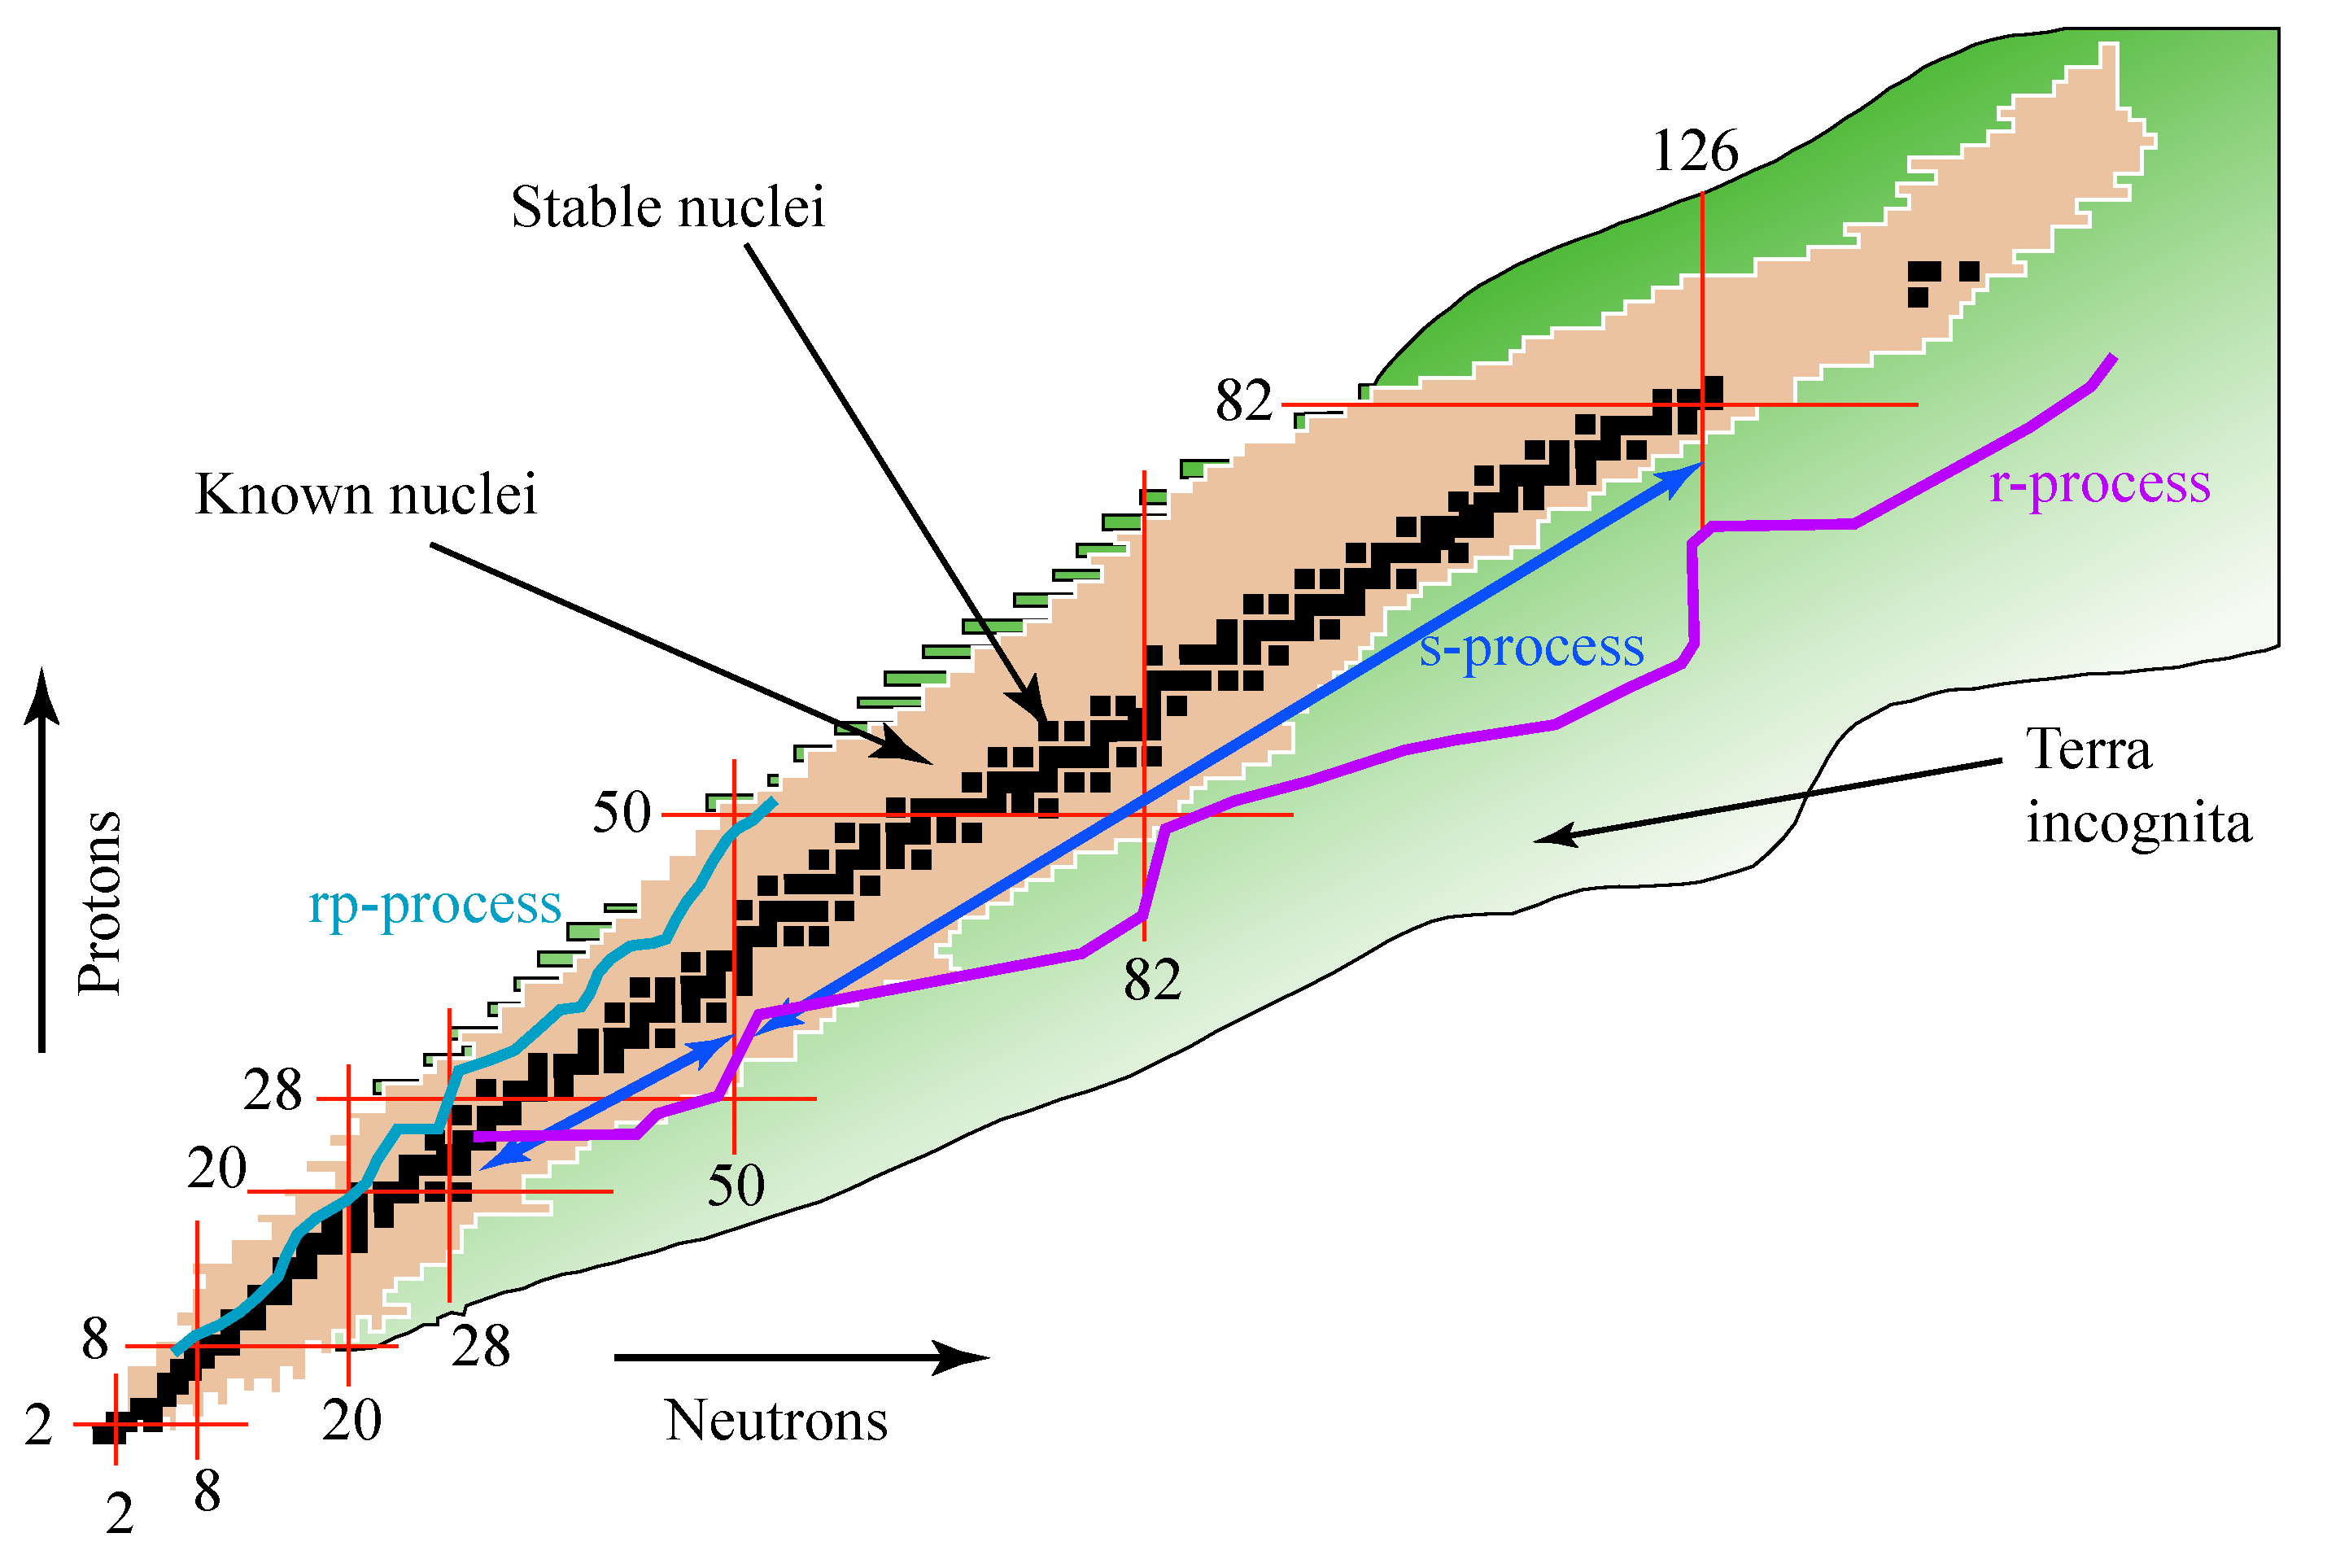
\includegraphics[width=\textwidth]{fig-timmes_table_nuclei02}\end{center}
 \caption{A chart of the nuclides showing the s- and r-process paths. Figure by \href{http://cococubed.asu.edu/pix_pages/nuclide_chart.shtml}{Frank Timmes}.}\label{fig:chartofnuclides}
\end{figure}

In the \rprocess, Fe-seed nuclei are bombarded with an extremely high flux of neutrons, which produces highly unstable neutron-rich isotopes out to the neutron drip line (at which neutrons can no longer be captured). This process, which is the only way to produce the heaviest elements such as Th and U, requires extremely high neutron densities of $10^{20}$--$10^{25}$ cm$^{-3}$ that most likely occur in the explosive conditions of core-collapse supernovae or neutron star mergers \citep[for a recent review of possible \rprocess sites, see][]{Thielemann:2011iy}. The \rprocess produces some of the most unstable nuclides in nature, so measurements of the lifetimes and decay channels of the relevant nuclei are extremely difficult to make with laboratory experiments. For this reason, the \rprocess component of an abundance distribution is often inferred from solar system material by subtracting the \sprocess component, which itself may be determined either theoretically \citep[e.g.,][]{Arlandini:1999eh,Goriely:1999wj,Sneden:2008cf} or empirically \citep[e.g.,][]{Simmerer:2004ib}. For this reason, improvements to our understanding of the \sprocess provide important constraints on the \rprocess.

The \sprocess refers to the opposite extreme of neutron capture rates, in which unstable nuclei typically have time to undergo $\beta^-$ decay before capturing a neutron. The \sprocess is far better understood than the \rprocess, and today we have a good qualitative picture of the \sprocess in nature \citep[e.g.,][]{Busso:1999ig,Herwig:2005jn,Karakas:2014jt}.

The \sprocess takes place in low- to intermediate-mass stars (with $M$ between about 0.8 and 8 \Msun) in the He-intershell region during the thermally pulsing \gls{AGB} phase \citep{Sanders:1967bm,Straniero:1995ed,Busso:1999ig}. Perhaps the clearest evidence of this is the detection of the unstable element Tc, whose longest-lived isotope has a half-life of 4.2 million years, in the atmospheres of AGB stars that are billions of years old \citep{Merrill:1952fi,Uttenthaler:2007hu}.

The \sprocess also takes place in massive stars \citep{Raiteri:1993ff}, which is discussed in Section \ref{sec:sprocessmassivestars}.

\subsection{The \sprocess in AGB stars}
The structure of an \gls{AGB} star is characterised by dual burning shells that surround a degenerate CO core. Outside of the CO core is a thin He-burning shell at the base of the He-rich intershell region. The He-rich intershell is surrounded by a H-burning shell beneath a hydrogen-rich deep convective envelope.

\begin{figure}
 \begin{center}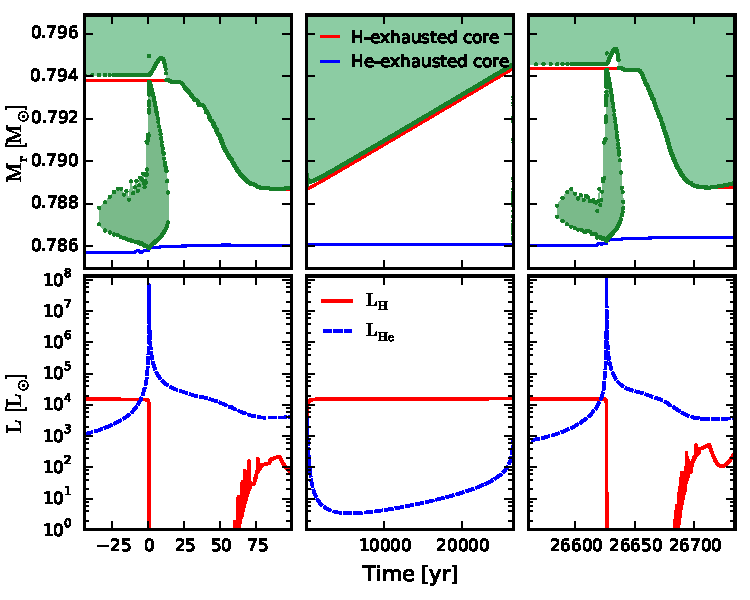
\includegraphics[width=\textwidth]{fig-tpcycle}\end{center}
 \caption{The AGB thermal pulse cycle illustrated with a 3 \Msun, $Z=0.0006$ model. Green shaded areas indicate convective regions. The style of the plot was inspired by \citet[][Figure 3]{Herwig:2005jn}.}\label{fig:tpcycle}
\end{figure}

The He-burning shell is thermally unstable, leading to a recurring series of structural changes every $10^2$--$10^5$ years that make up a thermal-pulse cycle. Figure \ref{fig:tpcycle} shows the first two thermal pulses in a 3 \Msun, $Z = 0.0006$ model\footnote{Here, $Z$ means the total mass fraction of all elements other than hydrogen and helium. Not to be confused with the atomic number $Z$.}. The He-burning shell ignites in a flash, a runaway reaction caused by a combination of the increasing temperature, the extreme temperature-sensitivity ($\epsilon \propto T^{40}$) of the triple-$\alpha$ reaction, and the lack of thermal regulation. The degeneracy and thinness of the He-burning shell prevent it from expanding sufficiently to quench the reaction until the luminosity has become very high \citep{Schwarzschild:1965dy,Weigert:1966th,Rose:1966bu}, often exceeding $10^8$ L$_\odot$ (as shown in the lower panel of Figure \ref{fig:tpcycle}). The steep temperature gradient produced by the shell flash leads to convective motions in the He-intershell, which becomes well-mixed.

The energy from the He-flash causes the star to expand, which pushes the H-burning shell outwards and extinguishes it. In the left-hand panel of Figure \ref{fig:tpcycle}, we can see that with the H-burning barrier removed, the lower boundary of the envelope convection zone can extend into the intershell, which is known as a `third dredge-up' (TDU) episode. The TDU transports nuclear burning products (such as \iso{12}{C} and \sprocess elements) to the stellar surface, where they affect the stellar spectrum and enrich the surrounding medium after being ejected by mass loss.

\begin{figure}
 \begin{center}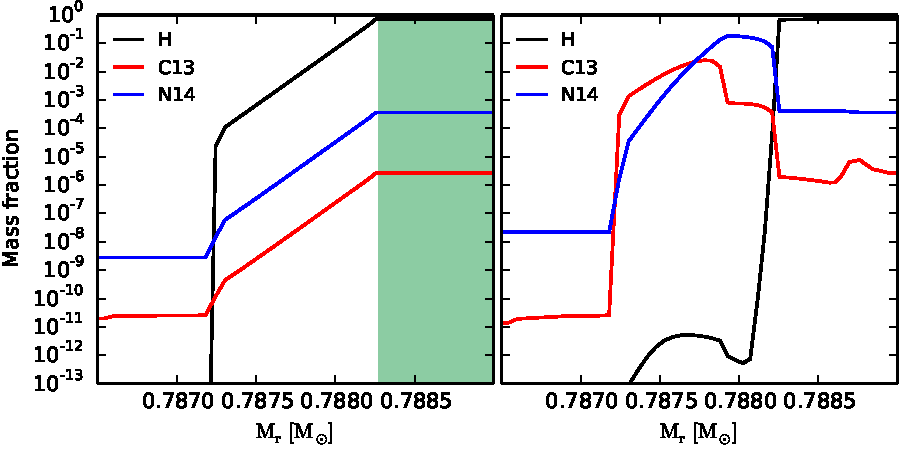
\includegraphics[width=\textwidth]{fig-c13pocket}\end{center}
 \caption{Composition profiles for H, \iso{13}{C}, and \iso{14}{N} showing the formation of a \iso{13}{C} pocket in a 3 \Msun, $Z=0.0006$ model with $\M{pmz}= 10^{-3}\,\Msun$. Left panel: Immediately after insertion the the protons as the convective envelope retreats (green shaded). Right panel: Approximately 1000 years later, a \iso{13}{C} pocket has formed below a \iso{14}{N} pocket.}\label{fig:c13pocket}
%first panel: T=2.8894745E+08 years
%second panel: T=2.8894858E+08 years
\end{figure}

Most of the free neutrons available for the \sprocess in low-mass ($\lesssim$ 3--4 \Msun) stars are produced via the $\iso{13}{C}(\alpha,n)\iso{16}{O}$ reaction under radiative conditions \citep{Cameron:1957eo,Scalo:1978ke,Straniero:1995ed,Gallino:1998eg}. Producing the seed \iso{13}{C} nuclei in stellar models requires the existence of a layer at the top of the \iso{12}{C}-rich intershell in which protons are `partially mixed' down from the envelope, thus enabling the CN cycle reaction $\iso{12}{C}(p,\gamma)\iso{13}{N}(\beta^+\nu)\iso{13}{C}$ to occur. The number of protons mixed into the region must be low because further proton capture completes the CN cycle to \iso{14}{N}, which is an efficient absorber of free neutrons.

The treatment of \iso{13}{C}-pocket formation in our models is shown in Figure \ref{fig:c13pocket}. The left-hand panel shows the exponential profile of protons that is added below the base of the envelope at the deepest extent of TDU. The right-hand panel, which displays the composition approximately 1000 years later, shows the resulting \iso{13}{C} pocket that forms below a pocket of \iso{14}{N}. The uncertainty surrounding the physical process that mixes protons into the intershell to form \iso{13}{C} pockets is a recurring theme in this thesis, and each of the main chapters go into further detail on this topic.

The major neutron source in intermediate-mass stars ($\gtrsim$ 4 \Msun) is the $\iso{22}{Ne}(\alpha,n)\allowbreak\iso{25}{Mg}$ reaction \citep{Iben:1975bn,Scalo:1978ke}. In the high temperatures of He-burning shell, \iso{22}{Ne} is produced via $\iso{14}{N}(\alpha,\gamma)\iso{18}{F}(\beta^+\nu)\iso{18}{O}(\alpha,\gamma)\iso{22}{Ne}$. Above temperatures of about $300\times 10^6$ K, the $\iso{22}{Ne}(\alpha,n)\iso{25}{Mg}$ reaction starts to become active, producing a burst of neutrons at the base of the intershell during convective pulses. An important byproduct of the \iso{22}{Ne} + $\alpha$ reactions is the production of \iso{25}{Mg} and \iso{26}{Mg}. These isotopes are particularly significant because Mg isotope ratios can be derived from the spectra of cool stars (with T$_\mathrm{eff}\lesssim 5000$ K), which can then be used to obtain clues about chemical evolution \citep[e.g.,][]{Yong:2003kb}.

\begin{figure}
 \begin{center}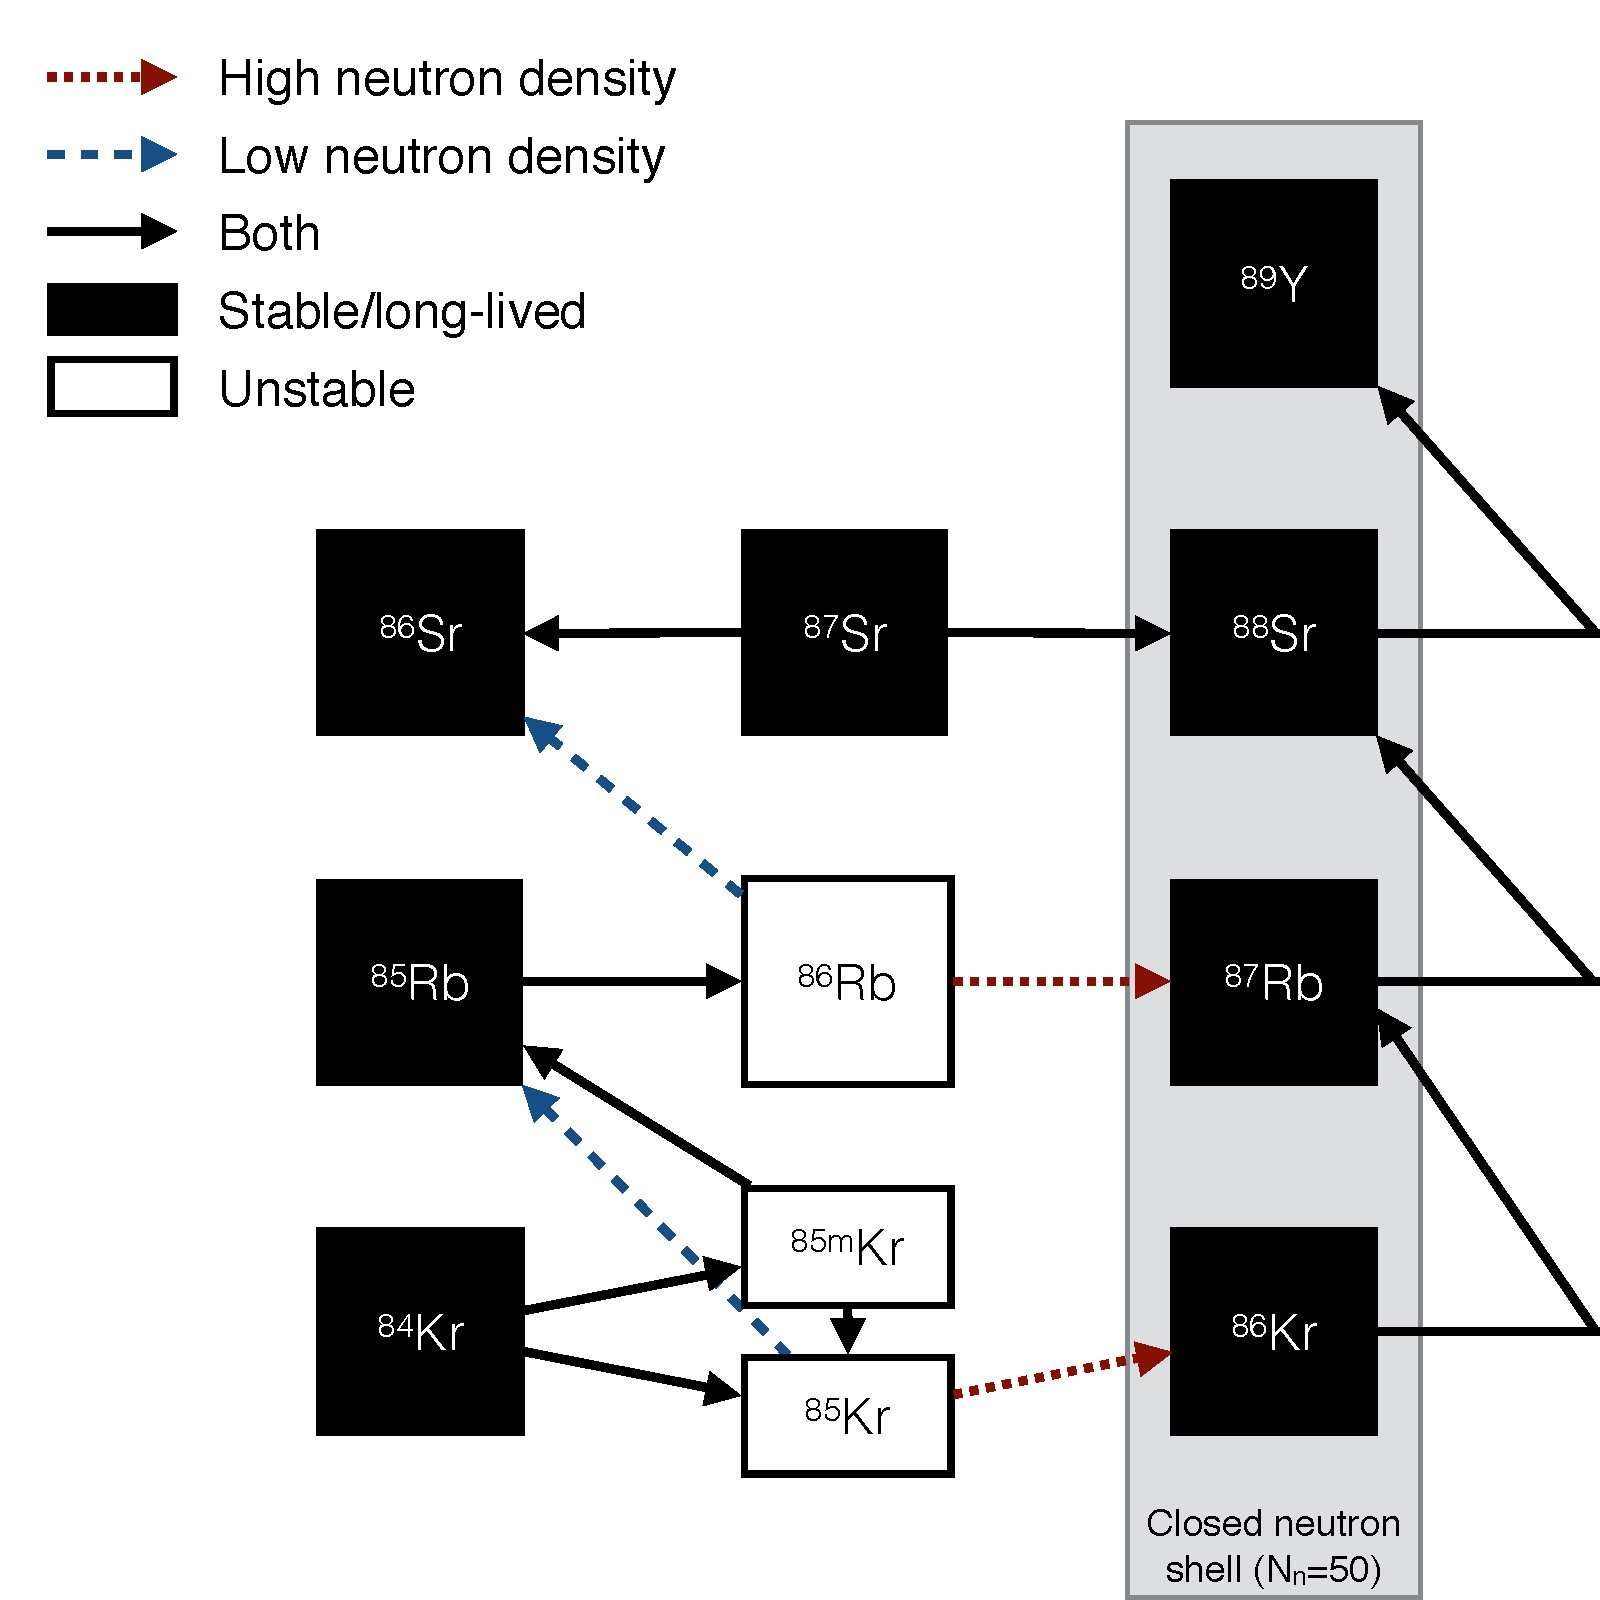
\includegraphics[width=0.9\textwidth]{fig-sprocessbranching}\end{center}
 \caption{The \sprocess path near the branchings at \iso{85}{Kr} and \iso{86}{Rb}. Similar to \citet[][Figure 1]{vanRaai:2012fq}}\label{fig:sprocessbranching}
\end{figure}

Another diagnostic of neutron-capture environments are the abundances of elements that are affected by \sprocess branching points \citep{Ward:1976ji}. Some unstable nuclides close to the valley of stability have half-lives on the order of days or years, resulting in $\beta$-decay rates that are similar to the neutron-capture rates. Two examples of nuclides with these immediate lifetimes are \iso{85}{Kr} ($\tau_{1/2}=$ 10.8 yr) and \iso{86}{Rb} ($\tau_{1/2}=$ 18.6 days) \citep{vanRaai:2012fq,Karakas:2012kc}. Figure \ref{fig:sprocessbranching} illustrates the different \sprocess paths near these nuclides that operate under high and low neutron densities. With neutron densities above $10^8$--$10^9$ cm$^\mathrm{-3}$, neutron captures on to \iso{85}{Kr} and \iso{86}{Rb} cause the \textit{s}-process path to produce \iso{87}{Rb}. \iso{87}{Rb} has a closed shell of neutrons, which gives it a very small neutron-capture cross section relative to \iso{85}{Rb} and neighbouring nuclides, causing it to accumulate \citep{Heil:2008kl}. At the high neutron densities resulting from the \iso{22}{Ne} neutron source, there is a larger production of Rb than Sr and Zr.

\begin{figure}
 \begin{center}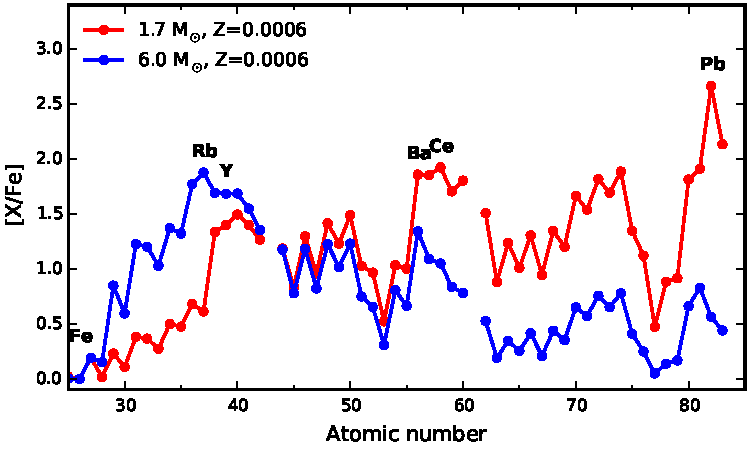
\includegraphics[width=\textwidth]{fig-agbfinalabund.pdf}\end{center}
 \caption[{Final [X/Fe] surface abundances (except for $Z=26$, which is [Fe/H]) for AGB models of 1.7 and 6.0 \Msun.}]{Final [X/Fe] surface abundances (except for $Z=26$, which is [Fe/H]) for AGB models of 1.7 and 6.0 \Msun. The 1.7 \Msun model is an example of \sprocess production via $\iso{13}{C}(\alpha,n)\iso{16}{O}$ reaction, and the 6 \Msun model of production via the $\iso{22}{Ne}(\alpha,n)\iso{25}{Mg}$ reaction.}\label{fig:agbfinalabund}
\end{figure}

Figure \ref{fig:agbfinalabund} shows the final surface abundances (in [X/Fe] notation\footnote{This is the standard spectroscopic abundance notation $[A/B] = \log_{10} (n_A/n_B)_{\star} - \log_{10} (n_A/n_B)_{\odot}$, where $\odot$ denotes the solar abundance ratio.}) of two example models with initial stellar masses of 1.7 and 6 \Msun, where the \sprocess production is dominated by the \iso{13}{C} and \iso{22}{Ne} neutron sources, respectively. The \sprocess in general tends to cause an accumulation of elements with stable isotopes whose neutrons form a closed shell configuration (magic numbers of neutrons), and therefore have a relatively small neutron-capture cross sections compared to their neighbours. The peak near Rb--Zr is caused by the accumulation of nuclides with 50 neutrons: \iso{87}{Rb}, \iso{88}{Sr}, \iso{89}{Y}, and \iso{90}{Zr}. A second peak forms around Ba--Ce due to nuclides with 82 neutrons: \iso{138}{Ba}, \iso{139}{La}, and \iso{140}{Ce}. A third peak forms at Pb due to the doubly-magic \iso{208}{Pb} nuclide with 82 protons and 126 neutrons.

In low-mass ($\lesssim$ 3 \Msun) stars such as the 1.7 \Msun model in Figure \ref{fig:agbfinalabund}, the \sprocess distribution is particularly enhanced near the Ba-peak elements and Pb \citep[as discussed in][]{Lugaro:2012ht}. In contrast, the \sprocess in intermediate-mass stars such as the 6 \Msun model results in a heavy-element distribution that is dominated by the first \sprocess peak near Sr, Y, and Zr. The effect of the \sprocess branching is evident in the 6 \Msun model from the enhancement in [Rb/Fe] relative to [(Sr,Y,Zr)/Fe].

After being dredged-up into the envelope via TDU, \sprocess nuclei are released into the surrounding medium by mass loss through stellar winds. The contribution of a particular chemical species $i$ (e.g., an element or nuclide) to the interstellar medium by a star over its lifetime is known as the stellar yield. We calculate this quantity using the formula
\begin{equation}
 M_{i}^\mathrm{yield} = \int_{0}^{\tau} X_i(t) \dot{M}(t) \,\mathrm{d}t,
\end{equation}
where $X_i(t)$ is the mass fraction of species $i$ at time $t$, $\dot{M}(t)$ is the stellar mass-loss rate at time $t$, and $\tau$ is the total stellar lifetime. For models with a non-zero envelope mass at the end of our calculations, we assume that all mass exterior to the core is ejected with the composition of the surface at the last computed model. A set of stellar yields are a prerequisite for constructing models of chemical evolution.

\section{Chemical Evolution}
Our knowledge of single stellar evolution and nucleosynthesis lays the groundwork for understanding chemical evolution, i.e., how the interstellar medium changes in chemical composition as it is enriched by dying stars. Observationally, the historical composition of the interstellar medium can be traced by low-mass stars. This is because of their extremely long lifetimes (tens of billions of years) and the fact that their atmospheres preserve their chemical compositions at birth, making them ideal 'stellar fossils'.

\subsection{Chemical evolution modelling}\label{sec:cemodelling}
By accounting for the major processes that affect star formation and the composition of the interstellar medium, we can construct theoretical models whose abundance evolution can be compared with the abundances from real stars measured by spectroscopy.

The basic components of a chemical evolution model are:
\begin{itemize}
\item initial conditions: the starting gas mass and chemical composition,
\item $\phi(m)$: the initial mass function,
\item $\psi$: the star formation rate (in \Msun/year) as a function of time or gas density,
\item $\tau(m)$: the stellar lifetime (in years) as a function of initial mass,
\item $m_{rem}(m)$: the remnant mass (in \Msun) as a function of initial mass, and
\item $q_i(m)$: the stellar yield of species $i$ from a star with initial mass $m$ (in \Msun).
\end{itemize}

The initial mass function is a distribution function for the initial masses of stars produced by star formation. For chemical evolution purposes, it is typically normalised such that $\phi(m) \,\ud m$ is the number of stars with masses between $m$ and $m + \ud m$ per \Msun of star formation. Common choices for the initial mass function include the classical \citet{Salpeter:1955hz} power law, or more recent forms such at the broken power law of \citet{Kroupa:1993tm}.

The star formation rate is often estimated by a power law function of the gas density \citep{Schmidt:1959bp,Kennicutt:2012ey} or even more simply, an exponentially decreasing rate that models a single initial burst.

The results from a grid of stellar evolution and nucleosynthesis models spanning a range of initial masses at the relevant metallicity are interpolated to fix several more of the required functions: the stellar lifetime function, the remnant mass function, and the stellar yields. We ignore the dependence on metallicity here for simplicity (and because star formation ends before the metallicity increases in our models), but more complex models can use interpolated yields from a grid that spans a range of metallicities.

With these ingredients, we can write a set of differential equations to be solved in order to model the chemical composition as a function of time. Here we describe a single-zone chemical evolution model for simplicity, although the model can be straightforwardly extended to multiple zones or two or three dimensional models. This would be achieved by solving the chemical evolution equations separately for each zone, with extra terms that account for the transfer of gas and stars across zone boundaries. The following summary of the equations of chemical evolution is based on \citet[][Chapter 7]{Pagel:2009ws}. 

The total mass of the system is the divided up into the gas mass ($g$) and the stellar mass ($s$). These variables evolve according to
\begin{align*}
	\frac{\ud s}{\ud t} &= \psi(t) - e(t),
\end{align*}
and
\begin{align*}
	\frac{\ud g}{\ud t} &= F(t) - E(t) + e(t) -  \psi(t),
\end{align*}
where $F$ is the galactic accretion rate, $E$ is the galactic ejection rate, $e$ is the rate of mass ejection from the stellar population, and $\psi$ is the star formation rate. The stellar mass ejection rate, $e(t)$ is
\begin{align*}
	e(t) &= \int_{m_{\tau=t}}^{m_U}(m-m_{rem}(m)) \, \psi(t-\tau(m)) \,\phi(m) \,\mathrm{d}m,
\end{align*}
where $m_{\tau=t}$ is the initial mass of a star with a lifetime of $t$, $m_U$ is the upper limit mass, $m_{rem}(m)$ is the mass of a remnant left by a star with an initial mass $m$, and $\tau(m)$ is the stellar lifetime.

For each chemical species $i$ the ejection rate is
\begin{align*}
	e_i(t) &= \int_{m_{\tau=t}}^{m_U} q_i(m) \, \psi(t-\tau(m))\,\phi(m) \,\mathrm{d}m,
\end{align*}
where $q_i(m)$ is the stellar yield of $i$ from a star with an initial mass of $m$.

The gas mass fractions $X_i(t)$ evolve according to:
\begin{align*}
	\frac{\ud}{\ud t}[g X_i] &= e_i - X_i\psi + X_{i,F}F - X_i E
\end{align*}
where $X_{i,F}$ represents the mass fraction of species $i$ in the in-falling material.

\subsection{Globular clusters}
Some of the oldest objects in the local universe are globular clusters, which are very dense, roughly spherical groups of about $10^5$--$10^6$ stars located mostly in the halo of galaxies. Our Milky Way galaxy hosts over 150 globular clusters \citep[][2010 edition]{Harris:1996fr} and many of these clusters are over ten billion years old \citep{Dotter:2009cq}.

Historically, the ages of globular clusters have provided a useful constraint on cosmology by setting a lower limit on the age of the universe \citep{Chaboyer:1996hh,Dotter:2010ek}. Their simplicity as single stellar populations has also made them extremely valuable for testing theories of stellar evolution \citep{Johnson:1955ec}, where a simple stellar population is defined as a group of stars that formed at the same time in a single burst of star formation within a gas cloud of a uniform chemical composition. The assumption that this described globular clusters made the age dating of clusters relatively straightforward; the age of the cluster is simply the lifetime of the stars that are currently leaving the main sequence, and these stars can be identified from a colour-magnitude diagram.

Detailed abundances studies have revealed that globular clusters show significant spreads in the abundances of light elements such as He, C, N, O, F, Na, Mg, and Al \citep{Cohen:1978gq,Peterson:1980ca,Gratton:2004dy}. The variations of these elements are correlated in a way that is almost exclusive to globular clusters \citep[i.e., it is rarely seen in field stars and open clusters, as shown by][]{Kraft:1982es,Shetrone:1996hp,Kraft:1997hp,Gratton:2000wg,DeSilva:2009ki} with anti-correlations between the abundances of C and N, Na and O, and sometimes Mg and Al \citep{Shetrone:1996hp}, typically with a C+N+O abundance that is constant within observational errors. These abundance patterns point to a H-burning process at high temperature ($\gtrsim80$ MK) and dilution with varying amounts of unprocessed material, although the stellar sites where this burning takes place and the mechanism of dilution are presently not understood \citep{Prantzos:2007bs}. Some current candidates for the hot hydrogen-burning environment are massive AGB (5--8 \Msun) stars \citep{Cottrell:1981ha,Ventura:2001ek}, rotating massive stars \citep{Prantzos:2006cv,Decressin:2007bf}, massive binaries \citep{deMink:2009kv,Bastian:2013fd}, and supermassive (>$10^4$ \Msun) stars \citep{Denissenkov:2014bc,Denissenkov:2015dw}.

The Milky Way globular clusters have metallicities ranging from [Fe/H] $\approx-2.4$ to $-0.3$, with remarkably little variation within each cluster in almost all cases. A survey of 19 globular clusters by \citet{Carretta:2009di} found no more than 0.05 dex scatter in [Fe/H] measurements, which is consistent with all of the clusters in their sample being mono-metallic.  There are a few ($\sim$ 10\%) exceptional clusters that do feature metallicity variation, and these are also some of the most massive clusters. Examples include M22, which has an intrinsic scatter in [Fe/H] of 0.10--0.15 dex \citep{Marino:2009je,DaCosta:2009jl} and $\omega$ Centauri, although the latter could be the tidally-stripped nucleus of a dwarf galaxy \citep{Freeman:1993vl,Bekki:2003dv} and might therefore formed differently to other globular clusters \citep[see the discussion in][]{Gratton:2004dy}.

The abundances of neutron-capture elements ($Z > 30$) are constant within most clusters \citep{Gratton:2004dy,Yong:2006ia,Yong:2008in,DOrazi:2010fs}. However, there are exceptions to this, including M15, which shows variations in \rprocess elements such as Eu \citep{Sneden:2000ba}. M22 shows two distinct populations with distinct abundances of \sprocess elements (Y, Zr, Ba) \citep{Marino:2009je,Villanova:2010ci}. Among globular clusters with constant abundances of neutron-capture elements, there exist cluster-to-cluster differences. For example, M4 is a fairly typical mono-metallic metal-poor GC ([Fe/H] $=-1.18$; \citealt{Carretta:2009di}), except that it has super-solar abundances of $s$-process peak elements \citep[e.g., Rb, Y, Zr, La, Ba, Pb;][]{Brown:1992dw,Ivans:1999hf}. This makes M4 more enriched with \sprocess elements than M5, another GC with a similar metallicity.

In Chapter \ref{chap:shinglesetal2014}, we will construct new chemical evolution models that incorporate yields from \gls{AGB} stars and rotating massive stars to investigate the internal \sprocess enrichment within the cluster M22, as well as the global \sprocess enrichment of M4.

\subsection{Chemical evolution code}
The candidate has developed a basic one-zone chemical evolution code in modern Fortran named `Evel ChemEvol'.

The Evel ChemEvol code solves the equations of chemical evolution (described in Section \ref{sec:cemodelling}) with a Simpson rule integration and an adaptive time step. To estimate the integration error at each step, the Simpson rule calculation is compared with a lower-order integration using the mid-point rule. If any of the integration stages exceed their configured error thresholds, the current step is recalculated with a shorter time step.

To ensure that the Evel ChemEvol code produces valid output, the software must be able to reproduce the results of an existing chemical evolution model. We chose to reproduce the model of the globular cluster NGC 6752 by \citet[][hereafter, F04]{Fenner:2004ju}.

\begin{figure}
 \begin{center}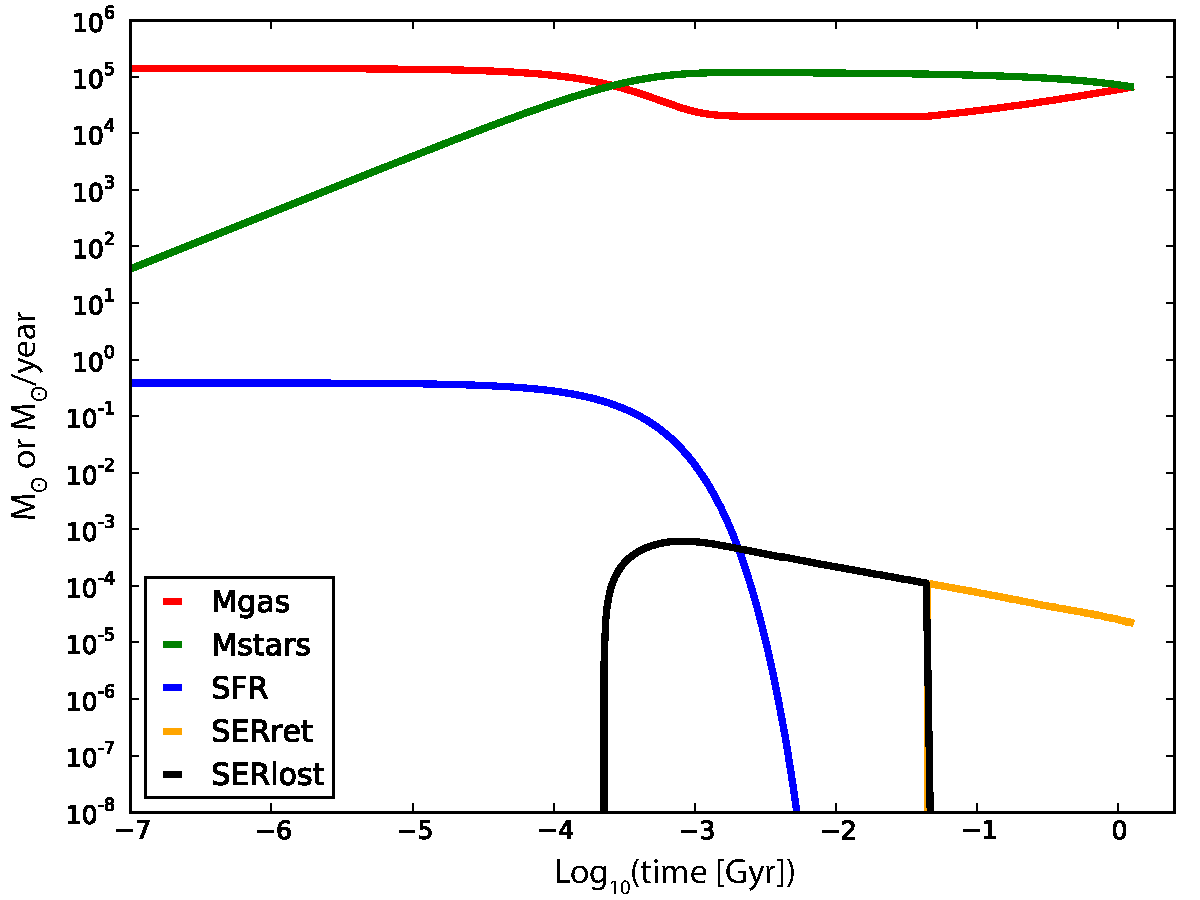
\includegraphics[width=\textwidth]{figures/cemodel}\end{center}
 \caption{Time evolution of Evel ChemEvol model variables. The plot shows the gas mass ($\M{gas}$, in \Msun), the stellar mass ($\M{stars}$, in \Msun), the star formation rate (SFR, in \Msun/yr), the stellar ejection rate of retained and lost ejecta (SERret and SERlost, in \Msun/yr). In this model, ejecta from stars < 6.5 \Msun is assumed to retained, while ejecta from more massive stars is lost.}\label{fig:cemodel}
\end{figure}

Following F04, the initial gas abundances are set by polluting primordial gas (roughly 75\% H and 25\% He) with the ejecta of massive stars until [Fe/H] increases to $-1.4$, the observed metallicity of NGC 6752. Many of initial these abundances were then manually adjusted to match F04, since the massive star yields of \citet{Kobayashi:2006fh} that we used were different to those of \citet{Chieffi:2002gl} that were used in F04. The initial gas mass is set to $1.4 \times 10^5$ \Msun, and star formation is triggered with an exponential falloff on a timescale of $10^7$ years. Figure \ref{fig:cemodel} illustrates the output of the chemical evolution model.

As shown in Figure \ref{fig:cemodel}, the stellar ejection rate is separated into retained ejecta from stars less massive than 6.5 \Msun, and ejecta from more massive stars, whose high-speed winds are assumed to escape the cluster system. The cutoff at 6.5 \Msun is chosen for consistency with F04.

\begin{figure*}
 \begin{center}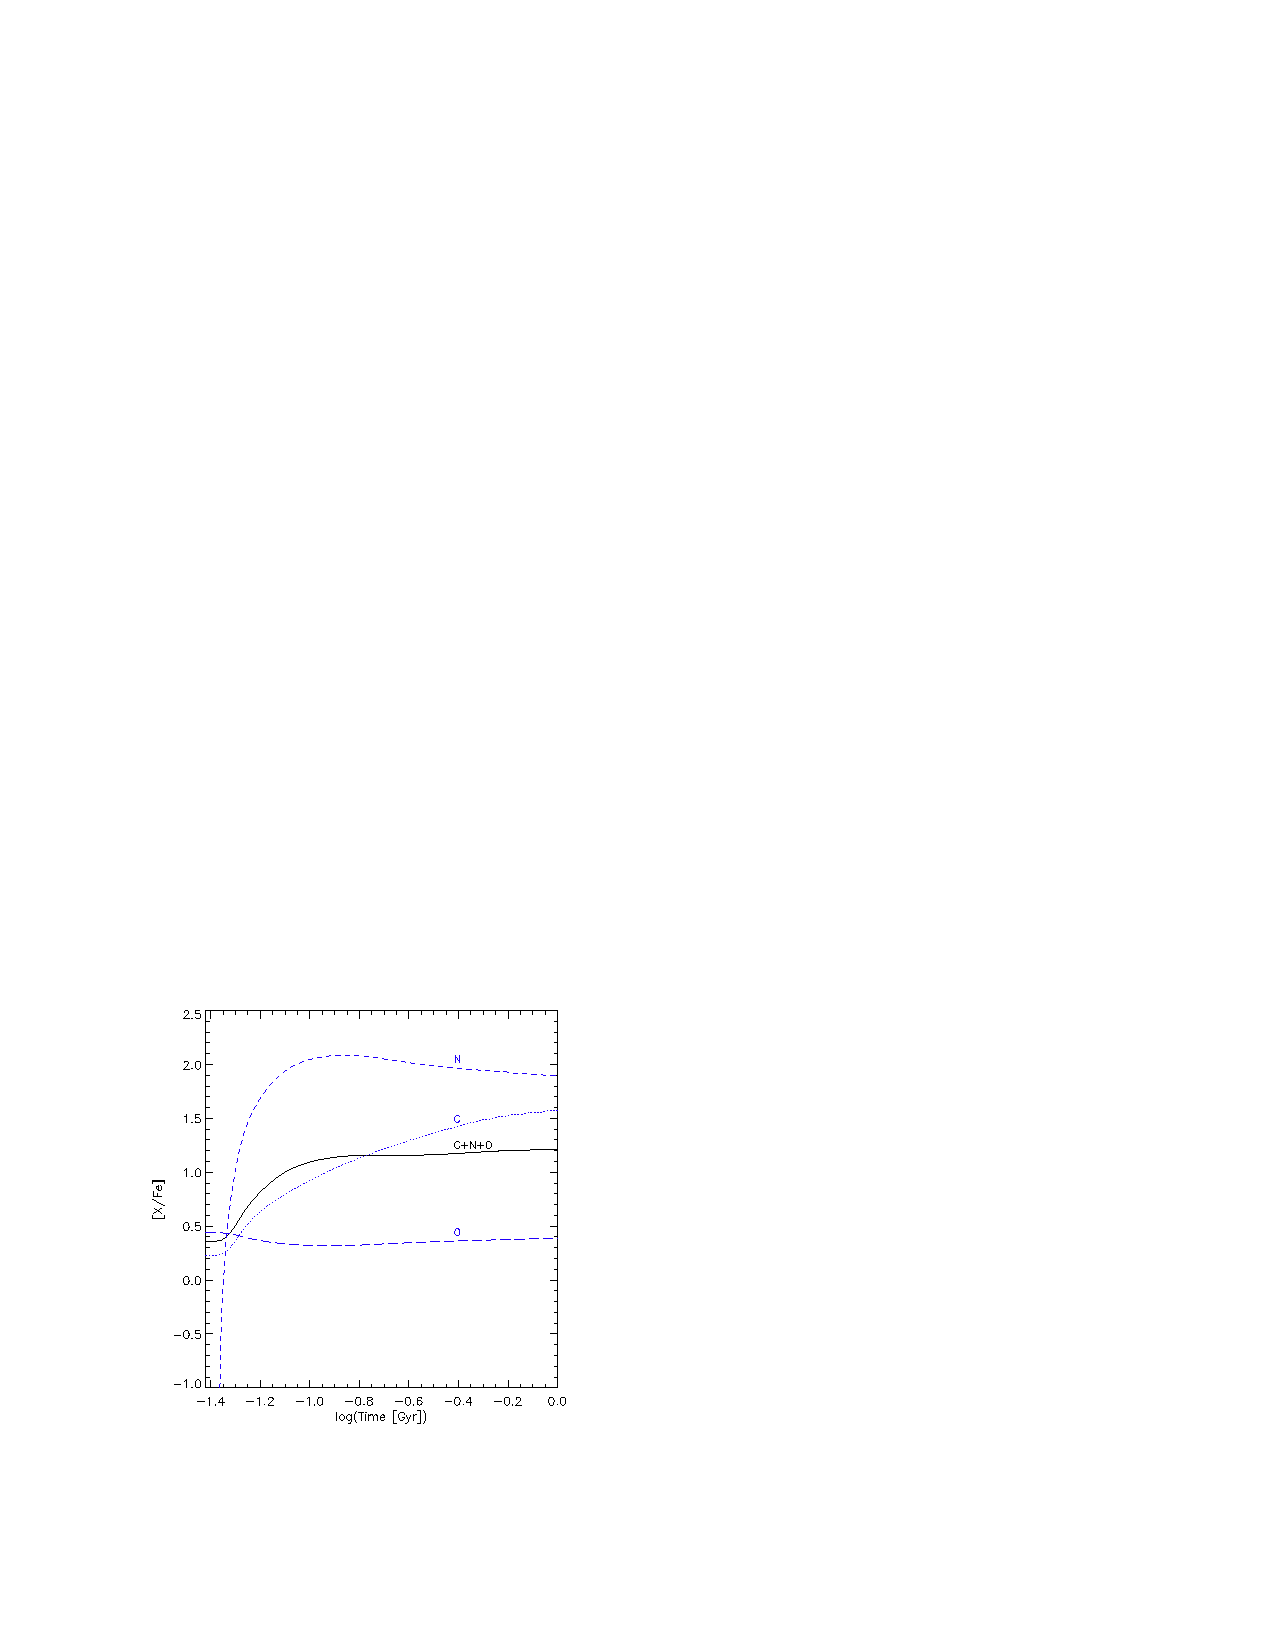
\includegraphics[height=0.45\textheight]{figures/Fenner04-CNO}\\
  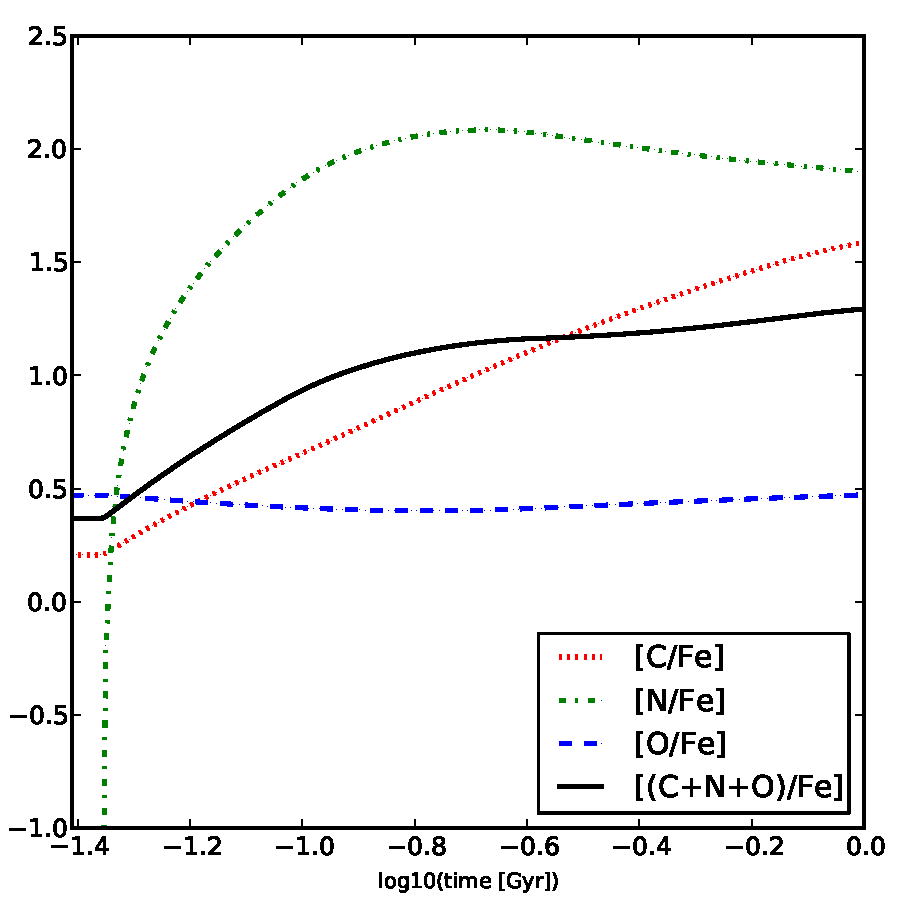
\includegraphics[height=0.45\textheight]{figures/cemodel-CNO}\end{center}
 \caption{Evolution of C, N, and O abundances from \citet{Fenner:2004ju} (top) and with Evel ChemEvol (bottom).}\label{fig:cemodel-cno}
\end{figure*}

\begin{figure}
 \begin{center}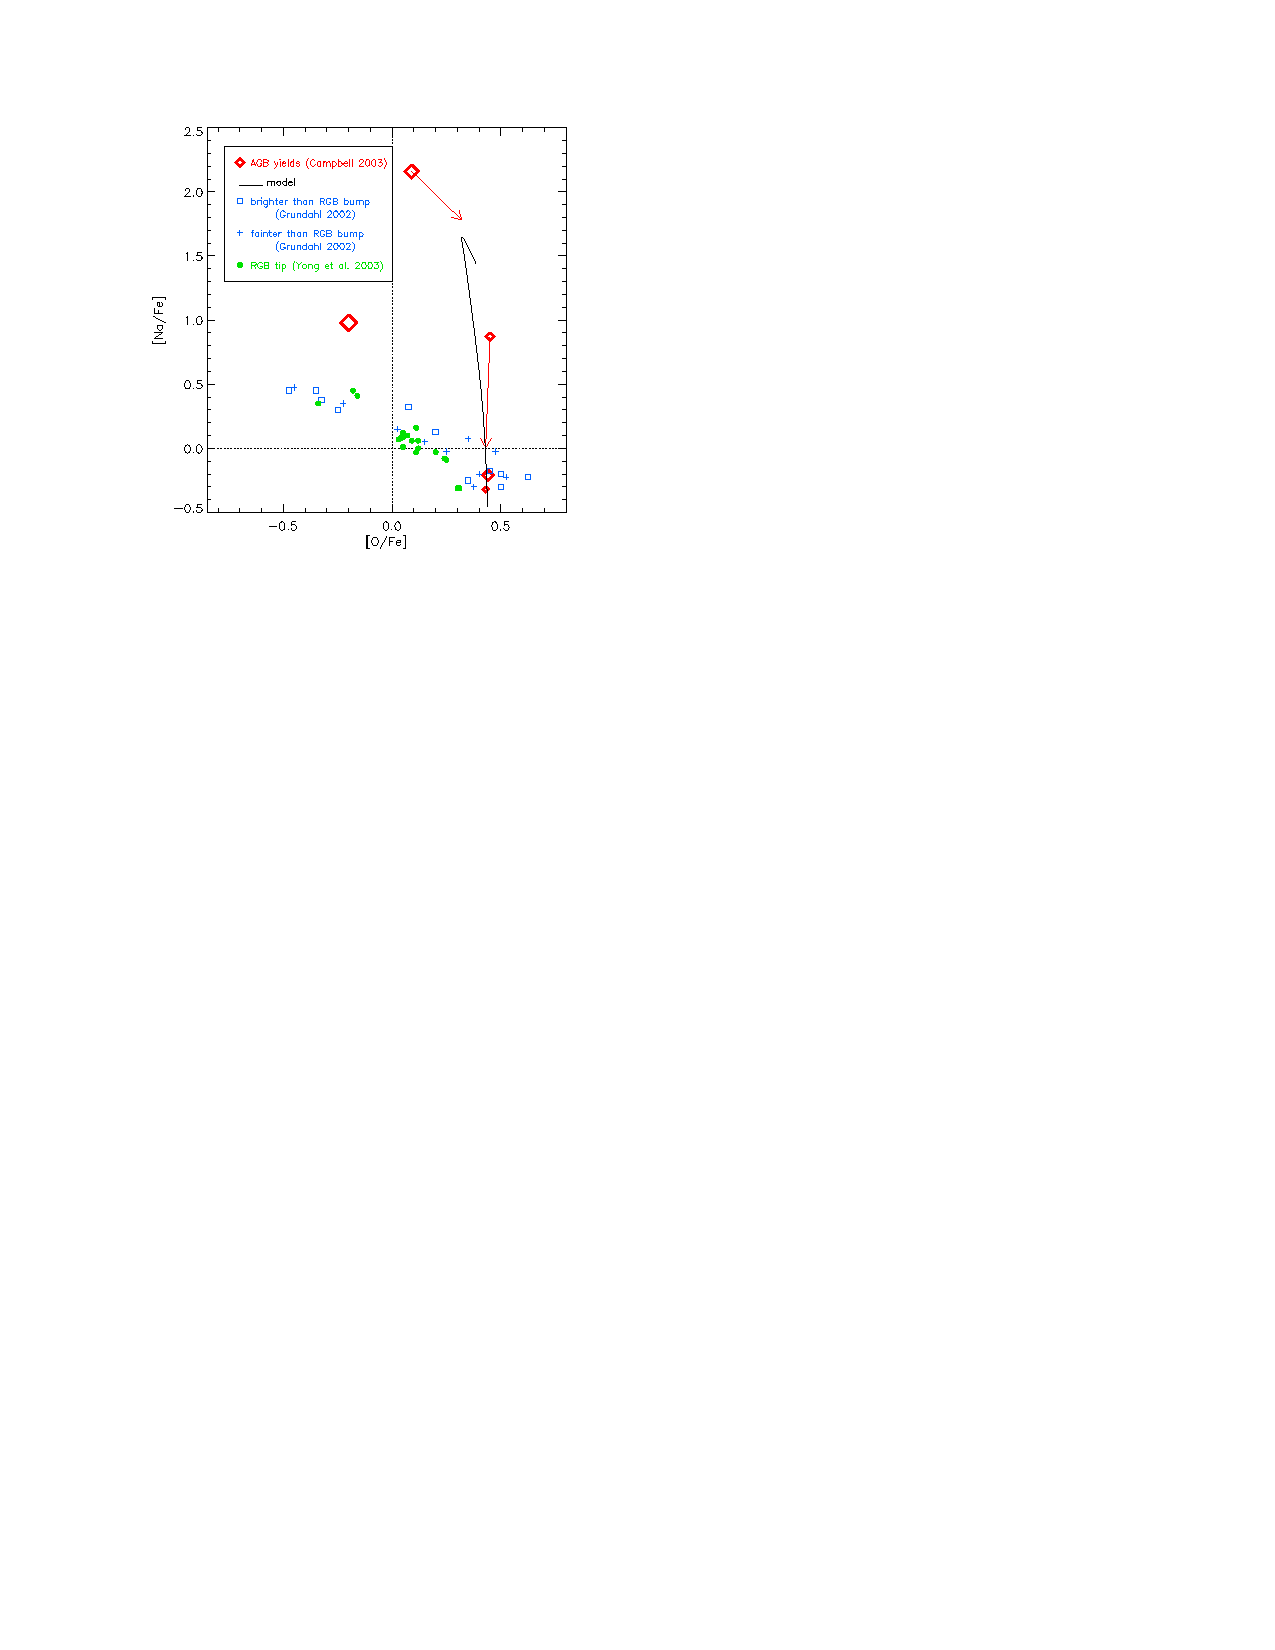
\includegraphics[height=0.45\textheight]{figures/Fenner04-Na-O}\\
 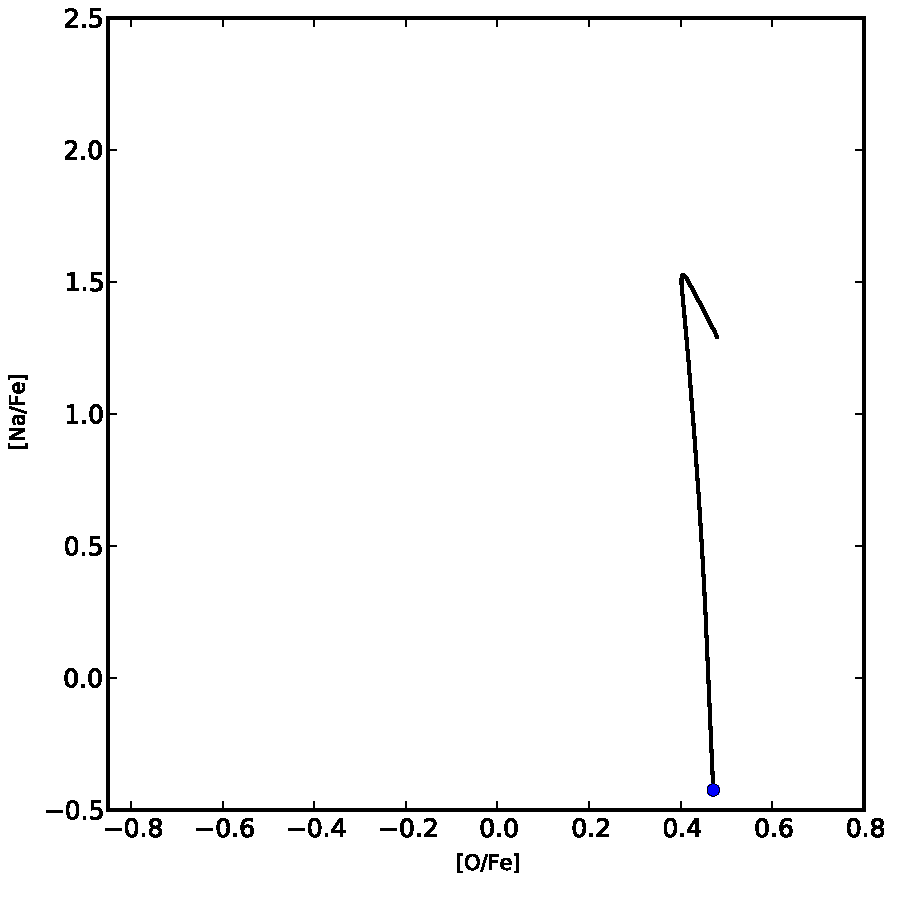
\includegraphics[height=0.45\textheight]{figures/cemodel-Na-O}\end{center}
 \caption{Evolution of Na and O abundances from \citet{Fenner:2004ju} (top) and with Evel ChemEvol (bottom).}\label{fig:cemodel-nao}
\end{figure}

\begin{figure}
 \begin{center}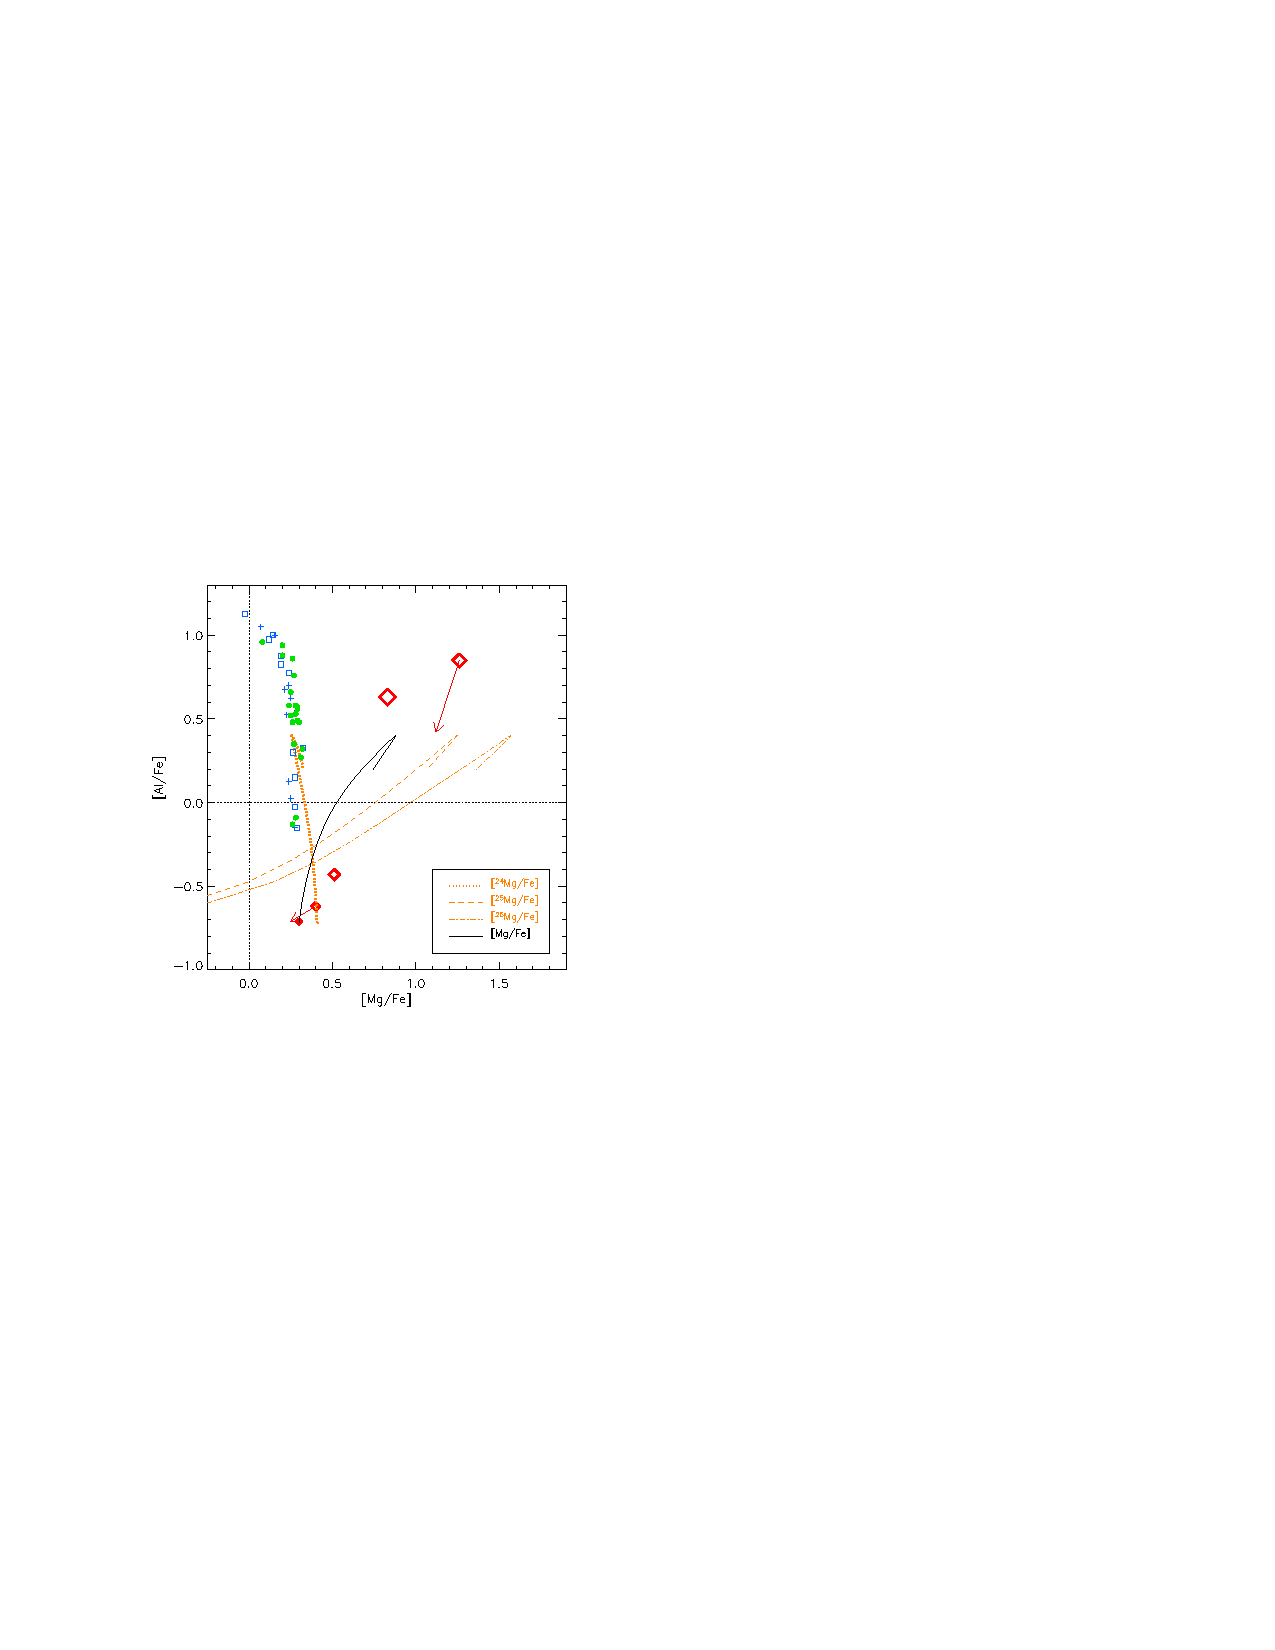
\includegraphics[height=0.45\textheight]{figures/Fenner04-Al-Mg}\\
 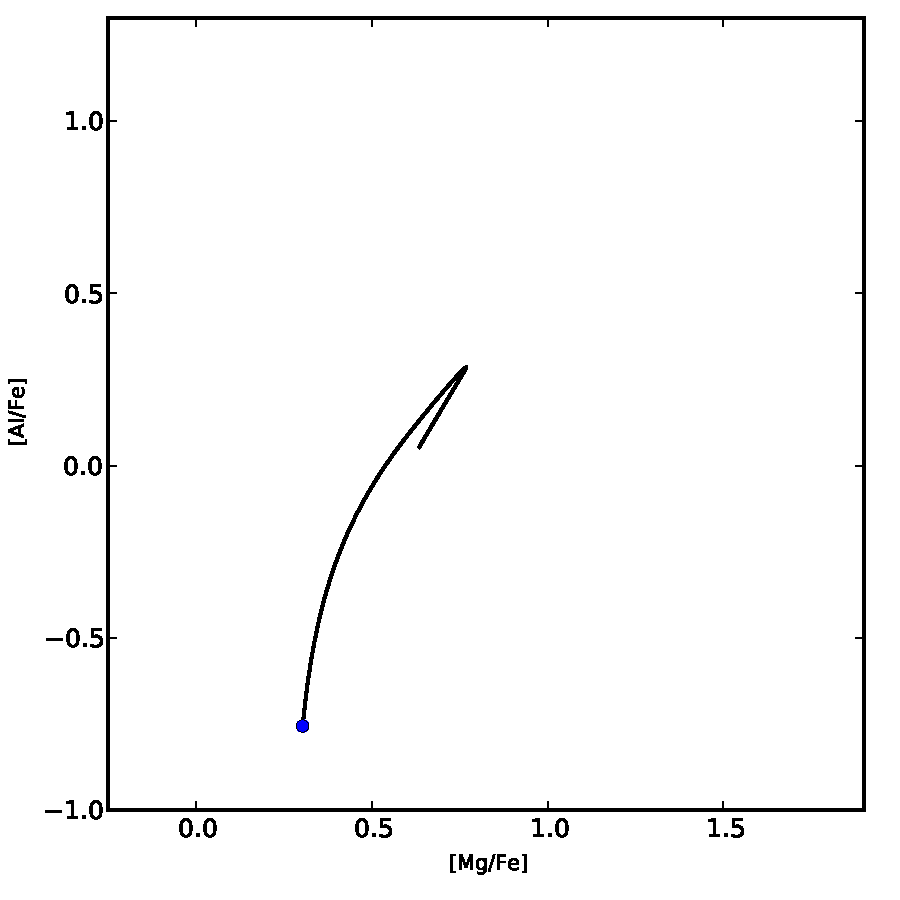
\includegraphics[height=0.45\textheight]{figures/cemodel-Al-Mg}\end{center}
 \caption{Evolution of Al and Mg abundances from \citet{Fenner:2004ju} (top) and with Evel ChemEvol (bottom).}\label{fig:cemodel-almg}
\end{figure}

We use the same \citet{Kroupa:1993tm} initial mass function and AGB stellar yields specified in F04. The stellar lifetime function is not described in F04 and is approximated here by a power law with the index $-2.9$. The results are in good agreement when assuming the same AGB yields for C, N, O (Figure \ref{fig:cemodel-cno}), Na and O (Figure \ref{fig:cemodel-nao}), and Al and Mg (Figure \ref{fig:cemodel-almg}).

\section{Outline of the Thesis}
This thesis presents new theoretical models of stellar evolution, nucleosynthesis, and chemical evolution, which we compare with observational data in the literature on planetary nebulae, post-AGB stars, and globular clusters.

We address the following questions:
\begin{itemize}
  \item Are the low sulphur abundances in planetary nebulae and post-AGB stars caused by nuclear reactions in their precursor AGB stars?
  \item How can we constrain the mixing process that forms \iso{13}{C} pockets in AGB stars?
  \item What is the origin of the \sprocess-rich material in M4 and M22?
  \item On what timescale did the \sprocess enrichment of M4 and M22 take place?
  \item How do high helium abundances affect the evolution, nucleosynthesis, and final fates of AGB stars?
  \item What are the chemical yields of He-rich intermediate-mass AGB stars?
\end{itemize}

Chapter \ref{chap:shingleskarakas2013} investigates the sulphur anomaly in planetary nebulae and post-AGB stars.

Chapter \ref{chap:shinglesetal2014} analyses the \sprocess enrichment of the globular clusters M4 and M22 using a chemical evolution code developed by the candidate.

Chapter \ref{chap:shinglesetal2015} focuses on the evolution and nucleosynthesis of stars with the high helium abundances found in globular cluster systems.

The main findings of these chapters are summarised in Chapter \ref{chap:conclusions}, where we also discuss the implications of this work and give some directions for future research.
